\section*{Problema 1}
Utilizamos el código para $N = 64$ y $N = 128$ utilizando el delta dado ($\dd{t} = 5\times 10^{-18}$)

\begin{multicols}{2}
\begin{figure}[H]
	\centering
	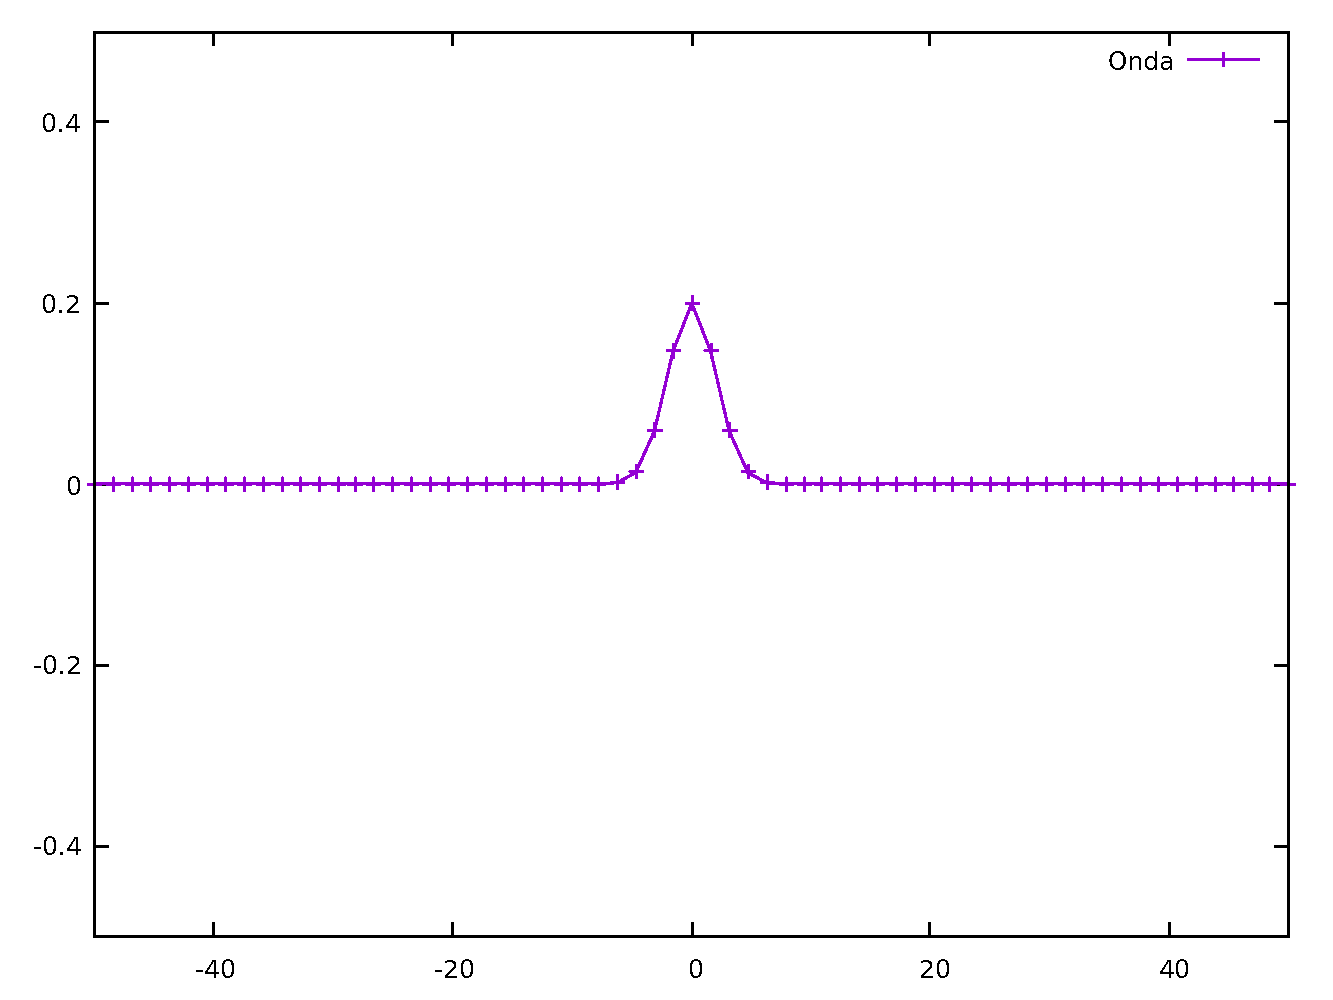
\includegraphics[scale=0.25]{../img/ej7-16_64.pdf}
	\caption{Amplitud de onda para $N = 64$.}
	\label{ej7-16_64}
\end{figure}

\begin{figure}[H]
	\centering
	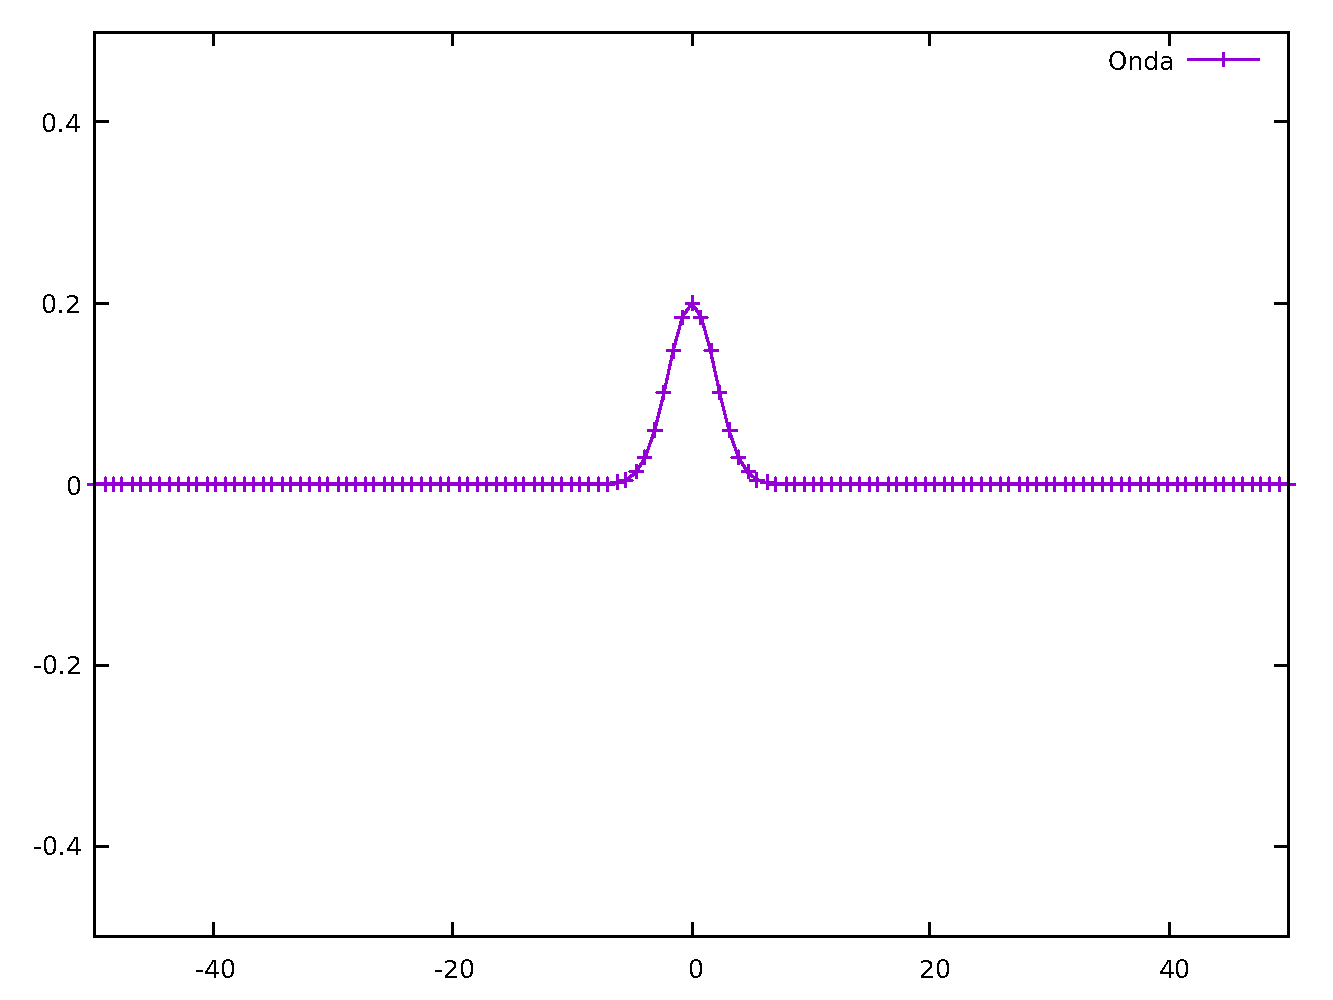
\includegraphics[scale=0.25]{../img/ej7-16_128.pdf}
	\caption{Amplitud de onda para $N = 128$.}
	\label{ej7-16_128}
\end{figure}
\end{multicols}


\begin{lstlisting}
// Librerias
#include <cmath>
#include <iostream>
#include <fstream>
#include <complex>
#include <iomanip>


using namespace std;



void output( complex<double> *u, double *x, double tiempo, int N, ostream &of );
void fourier( complex<double> *ftrans, complex<double> *f, int n );
void fourierInversa( complex<double> *f, complex<double> *ftrans, int n );


ofstream solucion;
complex<double> I(0.0, 1.0);

int main()
{
  int N = 128;
  int Niter = 100;
  int outCada = 1;
  double tiempo = 0.0;
  double L = 50.0;
  double k0 = 2*M_PI/(N+1);
  double hbar = sqrt(7.6199682);
  double masa = 1.0;
  double dx    = 2*L/N;
  double dt    = 5e-18;
  double delta_x = 2.0; // Ancho del paquete
  double k0momentum = sqrt(2*masa*2)/hbar;  // T=p^2/(2m), p=hbar*k
  solucion.open( "solucion.dat", ios::out );

  // Cantidades complejas
  complex<double> *psi, *trans, *phi, *expV, *expT;
  psi    = new complex<double>[ N+1 ];
  phi    = new complex<double>[ N+1 ];
  trans  = new complex<double>[ N+1 ];
  expV   = new complex<double>[ N+1 ];
  expT   = new complex<double>[ N+1 ];

  // Cantidades reales
  double *x, *k, *V;
  k = new double[ N+1 ];
  x = new double[ N+1 ];
  V = new double[ N+1 ];



  // Inicializar coordenada x
  for(int i=0; i<N+1; i++)
    x[i] = -L + i*dx;

  // Inicializar k
  for(int i=0; i<(N+1)/2; i++)
    k[i] = i*k0;

  for(int i=(N+1)/2; i<N+1; i++)
    k[i] = -k[N+1-i];


  // Inicializar Potencial
  for(int i=0; i<N+1; i++){
    if ( 20<=x[i] && x[i]<=30 )
      V[i] = 10.0;
    else
      V[i] = 0.0;

  }

  // Inicializar expomenciales de T y V
  for(int i=0; i<N+1; i++){
    expV[i] = exp( -I*V[i]*dt/(2*hbar) );
    expT[i] = exp( -I*hbar*k[i]*k[i]*dt/(2*masa) );
  }





  // condiciones iniciales
  for(int i=0; i<N+1; i++)
    psi[i] = exp(I*k0momentum*x[i] - x[i]*x[i]/pow(2*delta_x,2) )/pow(2*M_PI*pow(delta_x,2),0.25);


  // ciclo principal
  for(int j=0; j<=Niter; j++){

    if ( j%outCada==0 ){
      cout << "it = " << j << " / " << Niter << endl;;
      output( psi, x, tiempo, N, solucion );
    }


    // Aplicacion de los operadores
    for(int i=0; i<N+1; i++)
      phi[i] = expV[i] * psi[i];

    fourier( trans, phi, N+1 );

    for(int i=0; i<N+1; i++)
      phi[i] = expT[i] * trans[i];

    fourierInversa( psi, phi, N+1 );

    for(int i=0; i<N+1; i++)
      psi[i] = expV[i] * psi[i];


    // condiciones de frontera
    psi[0] = 0.0;
    psi[N] = 0.0;


    tiempo += dt;

  }

  return 0;
}



/***********************************************************************/



void output( complex<double> *psi, double *x, double tiempo, int N, ostream &of )
{
  for(int i=0; i<N+1; i++)
    of << tiempo << "\t" << x[i] << "\t"  << real(psi[i]) << "\t" << imag(psi[i]) << endl;

  of << endl << endl;
}



void fourier( complex<double> *ftrans, complex<double> *f, int n )
{
  for( int i=0; i<n+1; i++ ){
    ftrans[i] = 0.0;
    for( int j=0; j<n+1; j++ )
      ftrans[i] += f[j] * exp(-2*M_PI*I * (double)j * (double)i / (double)n);

    ftrans[i] /= sqrt(n);
  }
}


void fourierInversa( complex<double> *f, complex<double> *ftrans, int n )
{
  for( int i=0; i<n+1; i++ ){
    f[i] = 0.0;
    for( int j=0; j<n+1; j++ )
      f[i] += ftrans[j] * exp(2*M_PI*I*(double)j*(double)i/(double)n);

    f[i] /= sqrt(n);
  }
}


\end{lstlisting}


\section*{Problema 2}
Utilizando el mismo código, pero con energía inicial $E_o = 150 eV$ y realizamos $100$ pasos en el tiempo, con lo que tenemos las siguientes gráficas.

\begin{figure}[H]
	\centering
	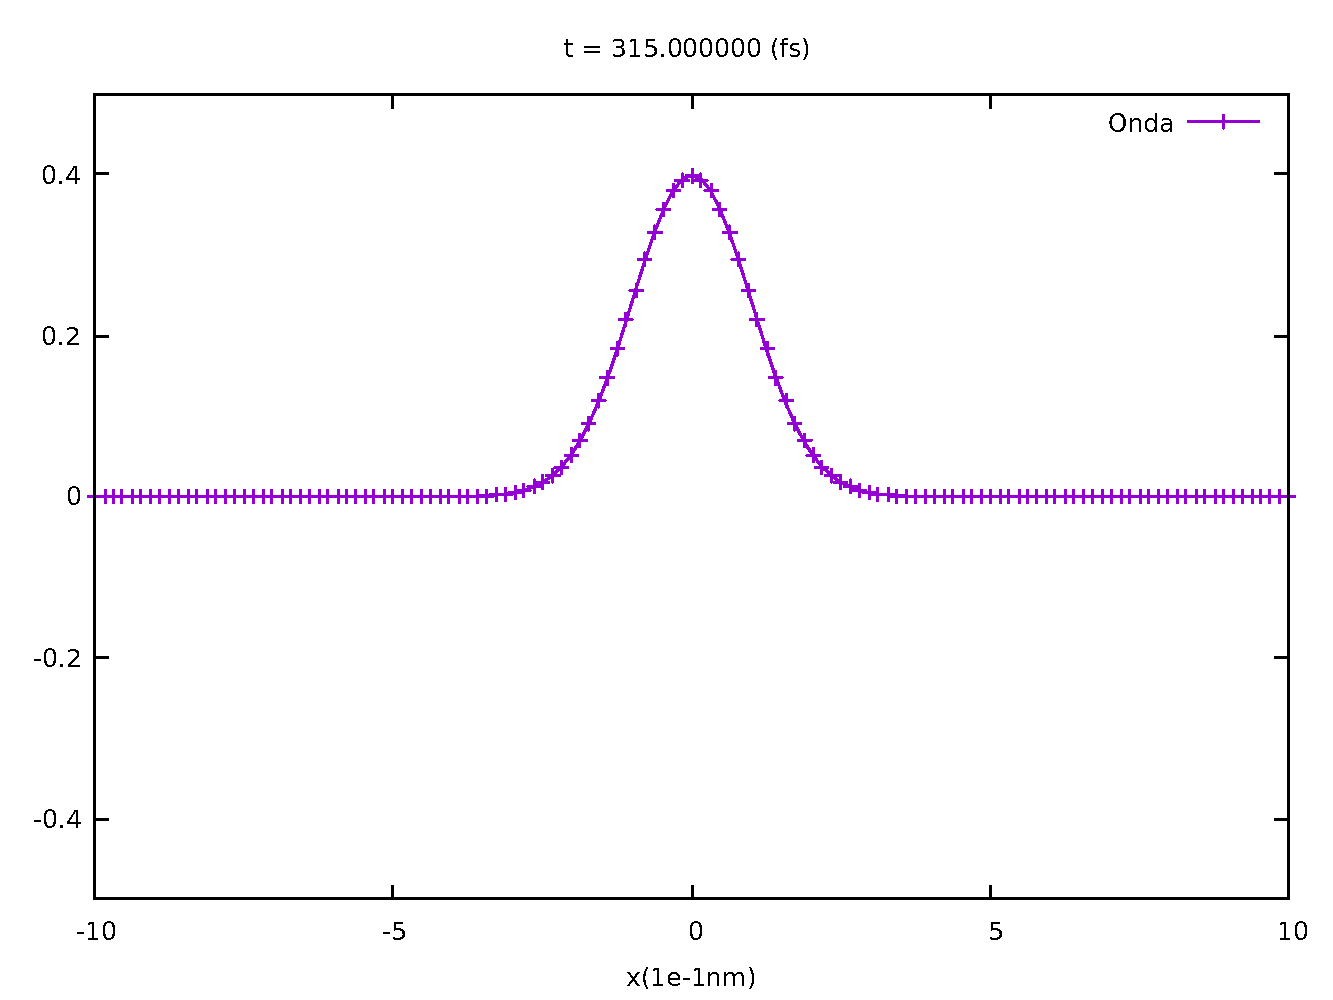
\includegraphics[scale=0.5]{../img/ej7-17.pdf}
	\caption{Onda para $E_o = 150 eV$.}
	\label{ej7-17}
\end{figure}

\begin{lstlisting}
// Librerias
#include <cmath>
#include <iostream>
#include <fstream>
#include <complex>
#include <iomanip>


using namespace std;



void output( complex<double> *u, double *x, double tiempo, int N, ostream &of );
void fourier( complex<double> *ftrans, complex<double> *f, int n );
void fourierInversa( complex<double> *f, complex<double> *ftrans, int n );


ofstream solucion;
complex<double> I(0.0, 1.0);

int main()
{
  int N = 128;
  int Niter = 100;
  int outCada = 1;
  double tiempo = 0.0;
  double L = 10.0;
  double k0 = 2*M_PI/(N+1);
  double hbar = sqrt(7.6199682);
  double masa = 1.0;
  double dx    = 2*L/N;
  double dt    = 5e-18;
  double delta_x = 1.0; // Ancho del paquete
  double k0momentum = sqrt(2*masa*150)/hbar;  // T=p^2/(2m), p=hbar*k
  solucion.open( "solucion.dat", ios::out );

  // Cantidades complejas
  complex<double> *psi, *trans, *phi, *expV, *expT;
  psi    = new complex<double>[ N+1 ];
  phi    = new complex<double>[ N+1 ];
  trans  = new complex<double>[ N+1 ];
  expV   = new complex<double>[ N+1 ];
  expT   = new complex<double>[ N+1 ];

  // Cantidades reales
  double *x, *k, *V;
  k = new double[ N+1 ];
  x = new double[ N+1 ];
  V = new double[ N+1 ];



  // Inicializar coordenada x
  for(int i=0; i<N+1; i++)
    x[i] = -L + i*dx;

  // Inicializar k
  for(int i=0; i<(N+1)/2; i++)
    k[i] = i*k0;

  for(int i=(N+1)/2; i<N+1; i++)
    k[i] = -k[N+1-i];


  // Inicializar Potencial
  for(int i=0; i<N+1; i++){
    if ( 20<=x[i] && x[i]<=30 )
      V[i] = 0.0;
    else
      V[i] = 0.0;

  }

  // Inicializar expomenciales de T y V
  for(int i=0; i<N+1; i++){
    expV[i] = exp( -I*V[i]*dt/(2*hbar) );
    expT[i] = exp( -I*hbar*k[i]*k[i]*dt/(2*masa) );
  }



  /* condiciones de frontera */
  //psi[0] = 0;
  //psi[N] = 0;


  // condiciones iniciales
  for(int i=0; i<N+1; i++)
    psi[i] = exp(I*k0momentum*x[i] - x[i]*x[i]/pow(2*delta_x,2) )/pow(2*M_PI*pow(delta_x,2),0.25);


  // ciclo principal
  for(int j=0; j<=Niter; j++){

    if ( j%outCada==0 ){
      cout << "it = " << j << " / " << Niter << endl;;
      output( psi, x, tiempo, N, solucion );
    }


    // Aplicacion de los operadores
    for(int i=0; i<N+1; i++)
      phi[i] = expV[i] * psi[i];

    fourier( trans, phi, N+1 );

    for(int i=0; i<N+1; i++)
      phi[i] = expT[i] * trans[i];

    fourierInversa( psi, phi, N+1 );

    for(int i=0; i<N+1; i++)
      psi[i] = expV[i] * psi[i];





    tiempo += dt;

  }

  return 0;
}



/***********************************************************************/



void output( complex<double> *psi, double *x, double tiempo, int N, ostream &of )
{
  for(int i=0; i<N+1; i++)
    of << tiempo << "\t" << x[i] << "\t"  << real(psi[i]) << "\t" << imag(psi[i]) << endl;

  of << endl << endl;
}



void fourier( complex<double> *ftrans, complex<double> *f, int n )
{
  for( int i=0; i<n+1; i++ ){
    ftrans[i] = 0.0;
    for( int j=0; j<n+1; j++ )
      ftrans[i] += f[j] * exp(-2*M_PI*I * (double)j * (double)i / (double)n);

    ftrans[i] /= sqrt(n);
  }
}


void fourierInversa( complex<double> *f, complex<double> *ftrans, int n )
{
  for( int i=0; i<n+1; i++ ){
    f[i] = 0.0;
    for( int j=0; j<n+1; j++ )
      f[i] += ftrans[j] * exp(2*M_PI*I*(double)j*(double)i/(double)n);

    f[i] /= sqrt(n);
  }
}

\end{lstlisting}













\section*{Problema 3}
Dada la barrera de potencial
	$$ V(x) = V_o ,\qquad \forall \quad x\geq 0, $$
y energía $E_o = 100eV$. Se tienen los siguientes resultados

\begin{figure}[H]
	\centering
	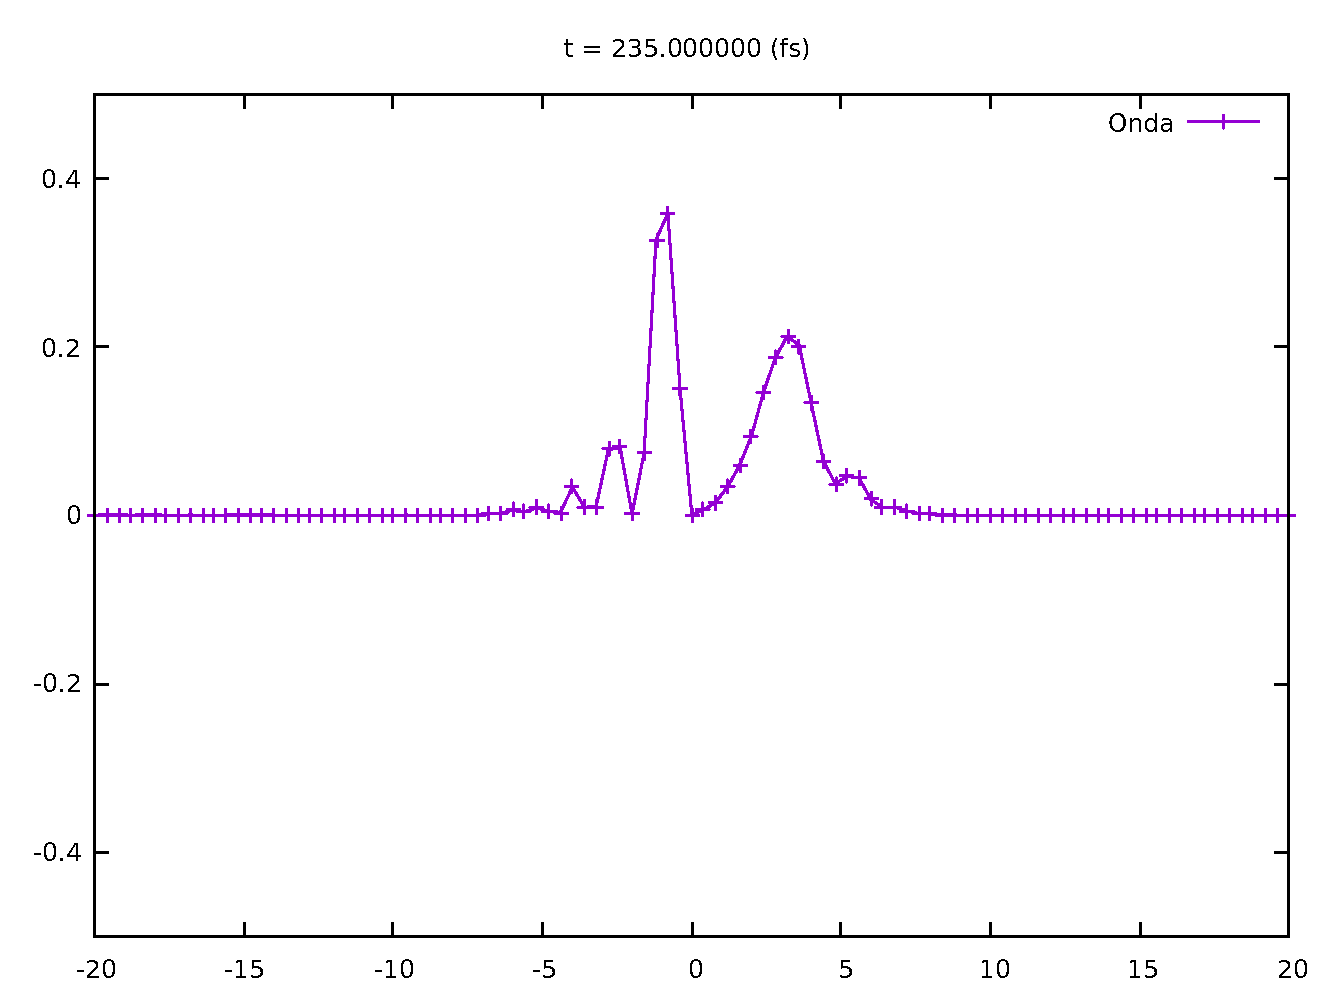
\includegraphics[scale=0.5]{../img/ej7-20.pdf}
	\caption{Onda con una barrera depotencial $V_o = 200eV$.}
	\label{ej7-20}
\end{figure}


\begin{lstlisting}
// Librerias
#include <cmath>
#include <iostream>
#include <fstream>
#include <complex>
#include <iomanip>


using namespace std;



void output( complex<double> *u, double *x, double tiempo, int N, ostream &of );
void fourier( complex<double> *ftrans, complex<double> *f, int n );
void fourierInversa( complex<double> *f, complex<double> *ftrans, int n );


ofstream solucion;
complex<double> I(0.0, 1.0);

int main()
{
  int N = 100;
  int Niter = 100;
  int outCada = 1;
  double tiempo = 0.0;
  double L = 20.0;
  double k0 = 2*M_PI/(N+1);
  double hbar = sqrt(7.6199682);
  double masa = 1.0;
  double dx    = 2*L/N;
  double dt    = 5e-2;
  double delta_x = 2.0; // Ancho del paquete
  double k0momentum = sqrt(2*masa*10)/hbar;  // T=p^2/(2m), p=hbar*k
  solucion.open( "solucion.dat", ios::out );

  // Cantidades complejas
  complex<double> *psi, *trans, *phi, *expV, *expT;
  psi    = new complex<double>[ N+1 ];
  phi    = new complex<double>[ N+1 ];
  trans  = new complex<double>[ N+1 ];
  expV   = new complex<double>[ N+1 ];
  expT   = new complex<double>[ N+1 ];

  // Cantidades reales
  double *x, *k, *V;
  k = new double[ N+1 ];
  x = new double[ N+1 ];
  V = new double[ N+1 ];



  // Inicializar coordenada x
  for(int i=0; i<N+1; i++)
    x[i] = -L + i*dx;

  // Inicializar k
  for(int i=0; i<(N+1)/2; i++)
    k[i] = i*k0;

  for(int i=(N+1)/2; i<N+1; i++)
    k[i] = -k[N+1-i];


  // Inicializar Potencial
  for(int i=0; i<N+1; i++){
    if ( 0<=x[i] && x[i]<=20 )
      V[i] = 200.0;
    else
      V[i] = 0.0;

  }

  // Inicializar expomenciales de T y V
  for(int i=0; i<N+1; i++){
    expV[i] = exp( -I*V[i]*dt/(2*hbar) );
    expT[i] = exp( -I*hbar*k[i]*k[i]*dt/(2*masa) );
  }



  /* condiciones de frontera */
  //psi[0] = 0;
  //psi[N] = 0;


  // condiciones iniciales
  for(int i=0; i<N+1; i++)
    psi[i] = exp(I*k0momentum*x[i] - x[i]*x[i]/pow(2*delta_x,2) )/pow(2*M_PI*pow(delta_x,2),0.25);


  // ciclo principal
  for(int j=0; j<=Niter; j++){

    if ( j%outCada==0 ){
      cout << "it = " << j << " / " << Niter << endl;;
      output( psi, x, tiempo, N, solucion );
    }


    // Aplicacion de los operadores
    for(int i=0; i<N+1; i++)
      phi[i] = expV[i] * psi[i];

    fourier( trans, phi, N+1 );

    for(int i=0; i<N+1; i++)
      phi[i] = expT[i] * trans[i];

    fourierInversa( psi, phi, N+1 );

    for(int i=0; i<N+1; i++)
      psi[i] = expV[i] * psi[i];


    // condiciones de frontera
    psi[0] = 0.0;
    psi[N] = 0.0;


    tiempo += dt;

  }

  return 0;
}



/***********************************************************************/



void output( complex<double> *psi, double *x, double tiempo, int N, ostream &of )
{
  for(int i=0; i<N+1; i++)
    of << tiempo << "\t" << x[i] << "\t"  << real(psi[i]) << "\t" << imag(psi[i]) << endl;

  of << endl << endl;
}



void fourier( complex<double> *ftrans, complex<double> *f, int n )
{
  for( int i=0; i<n+1; i++ ){
    ftrans[i] = 0.0;
    for( int j=0; j<n+1; j++ )
      ftrans[i] += f[j] * exp(-2*M_PI*I * (double)j * (double)i / (double)n);

    ftrans[i] /= sqrt(n);
  }
}


void fourierInversa( complex<double> *f, complex<double> *ftrans, int n )
{
  for( int i=0; i<n+1; i++ ){
    f[i] = 0.0;
    for( int j=0; j<n+1; j++ )
      f[i] += ftrans[j] * exp(2*M_PI*I*(double)j*(double)i/(double)n);

    f[i] /= sqrt(n);
  }
}

\end{lstlisting}









\section*{Problema 4}
Dados los mismos datos que el ejercicio anterior, pero con $E_o = 225eV$.


\begin{figure}[H]
	\centering
	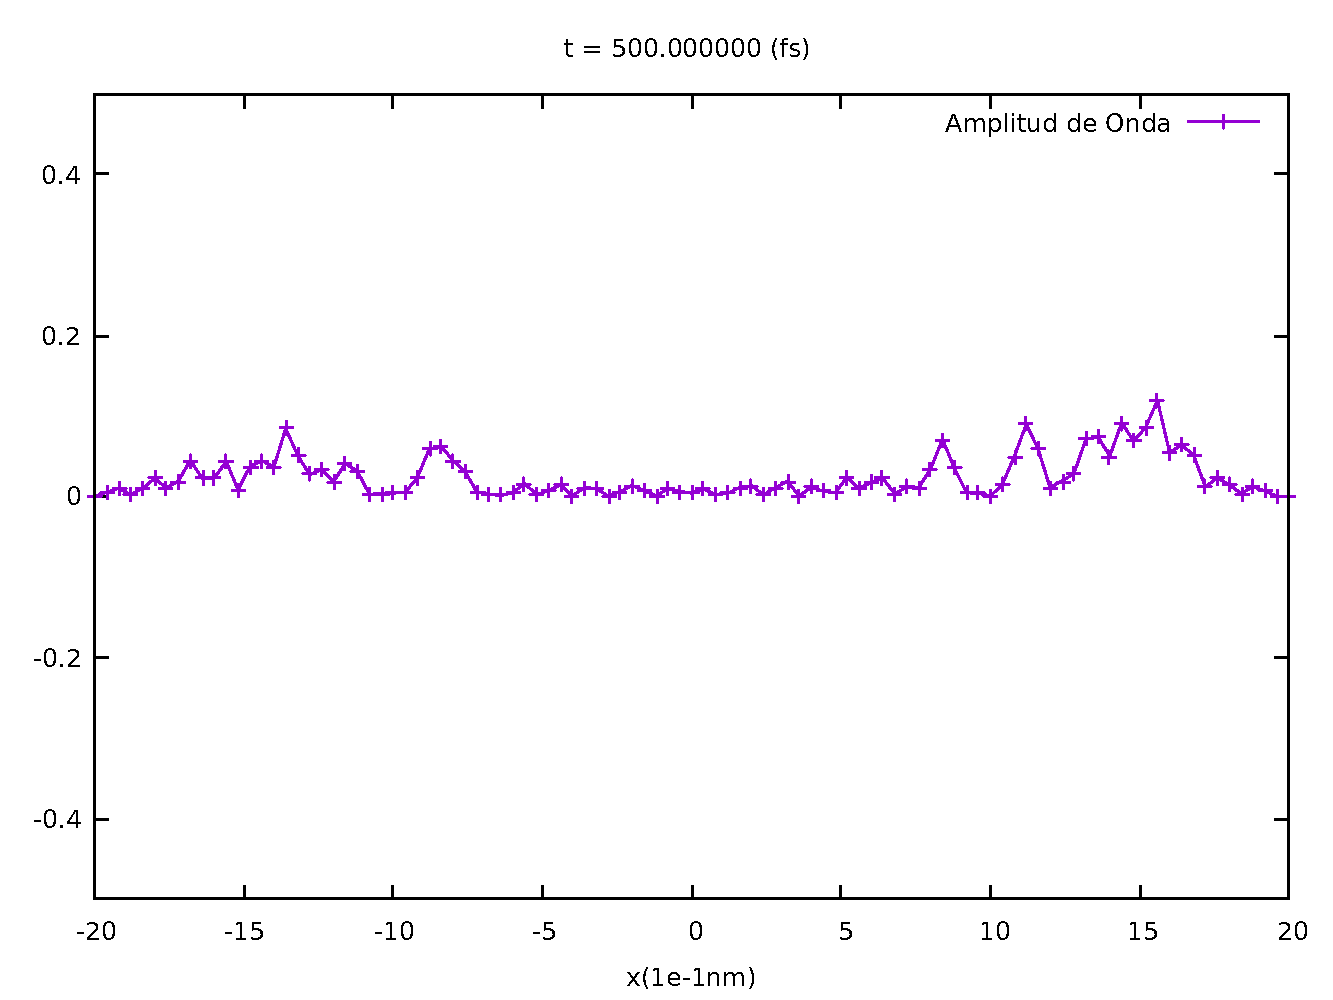
\includegraphics[scale=0.5]{../img/ej7-22.pdf}
	\caption{Onda con una barrera depotencial $V_o = 200eV$, pero con una energía inicial de $225eV$. Con esto se ve claro que parte de la onda supera dicha barrera de potencial.}
	\label{ej7-22}
\end{figure}


\begin{lstlisting}
// Librerias
#include <cmath>
#include <iostream>
#include <fstream>
#include <complex>
#include <iomanip>


using namespace std;



void output( complex<double> *u, double *x, double tiempo, int N, ostream &of );
void fourier( complex<double> *ftrans, complex<double> *f, int n );
void fourierInversa( complex<double> *f, complex<double> *ftrans, int n );


ofstream solucion;
complex<double> I(0.0, 1.0);

int main()
{
  int N = 100;
  int Niter = 100;
  int outCada = 1;
  double tiempo = 0.0;
  double L = 20.0;
  double k0 = 2*M_PI/(N+1);
  double hbar = sqrt(7.6199682);
  double masa = 1.0;
  double dx    = 2*L/N;
  double dt    = 5e-2;
  double delta_x = 1.0; // Ancho del paquete
  double k0momentum = sqrt(2*masa*225)/hbar;  // T=p^2/(2m), p=hbar*k
  solucion.open( "solucion.dat", ios::out );

  // Cantidades complejas
  complex<double> *psi, *trans, *phi, *expV, *expT;
  psi    = new complex<double>[ N+1 ];
  phi    = new complex<double>[ N+1 ];
  trans  = new complex<double>[ N+1 ];
  expV   = new complex<double>[ N+1 ];
  expT   = new complex<double>[ N+1 ];

  // Cantidades reales
  double *x, *k, *V;
  k = new double[ N+1 ];
  x = new double[ N+1 ];
  V = new double[ N+1 ];



  // Inicializar coordenada x
  for(int i=0; i<N+1; i++)
    x[i] = -L + i*dx;

  // Inicializar k
  for(int i=0; i<(N+1)/2; i++)
    k[i] = i*k0;

  for(int i=(N+1)/2; i<N+1; i++)
    k[i] = -k[N+1-i];


  // Inicializar Potencial
  for(int i=0; i<N+1; i++){
    if ( 0<=x[i] && x[i]<=20 )
      V[i] = 200.0;
    else
      V[i] = 0.0;

  }

  // Inicializar expomenciales de T y V
  for(int i=0; i<N+1; i++){
    expV[i] = exp( -I*V[i]*dt/(2*hbar) );
    expT[i] = exp( -I*hbar*k[i]*k[i]*dt/(2*masa) );
  }



  /* condiciones de frontera */
  //psi[0] = 0;
  //psi[N] = 0;


  // condiciones iniciales
  for(int i=0; i<N+1; i++)
    psi[i] = exp(I*k0momentum*x[i] - x[i]*x[i]/pow(2*delta_x,2) )/pow(2*M_PI*pow(delta_x,2),0.25);


  // ciclo principal
  for(int j=0; j<=Niter; j++){

    if ( j%outCada==0 ){
      cout << "it = " << j << " / " << Niter << endl;;
      output( psi, x, tiempo, N, solucion );
    }


    // Aplicacion de los operadores
    for(int i=0; i<N+1; i++)
      phi[i] = expV[i] * psi[i];

    fourier( trans, phi, N+1 );

    for(int i=0; i<N+1; i++)
      phi[i] = expT[i] * trans[i];

    fourierInversa( psi, phi, N+1 );

    for(int i=0; i<N+1; i++)
      psi[i] = expV[i] * psi[i];





    tiempo += dt;

  }

  return 0;
}



/***********************************************************************/






void output( complex<double> *psi, double *x, double tiempo, int N, ostream &of )
{
  for(int i=0; i<N+1; i++)
    of << tiempo << "\t" << x[i] << "\t"  << real(psi[i]) << "\t" << imag(psi[i]) << endl;

  of << endl << endl;
}



void fourier( complex<double> *ftrans, complex<double> *f, int n )
{
  for( int i=0; i<n+1; i++ ){
    ftrans[i] = 0.0;
    for( int j=0; j<n+1; j++ )
      ftrans[i] += f[j] * exp(-2*M_PI*I * (double)j * (double)i / (double)n);

    ftrans[i] /= sqrt(n);
  }
}


void fourierInversa( complex<double> *f, complex<double> *ftrans, int n )
{
  for( int i=0; i<n+1; i++ ){
    f[i] = 0.0;
    for( int j=0; j<n+1; j++ )
      f[i] += ftrans[j] * exp(2*M_PI*I*(double)j*(double)i/(double)n);

    f[i] /= sqrt(n);
  }
}

\end{lstlisting}









\section*{Problema 5}
Ahora, se tiene un pozo de potencial con $V_o = -200eV$ en el rango de $0 \leq x \leq a$, $a = 1.963A$ y $-30A \leq x \leq 30A$. Con esto se tienen las siguientes gráficas de la onda pasando por el pozo

\begin{multicols}{2}
\begin{figure}[H]
	\centering
	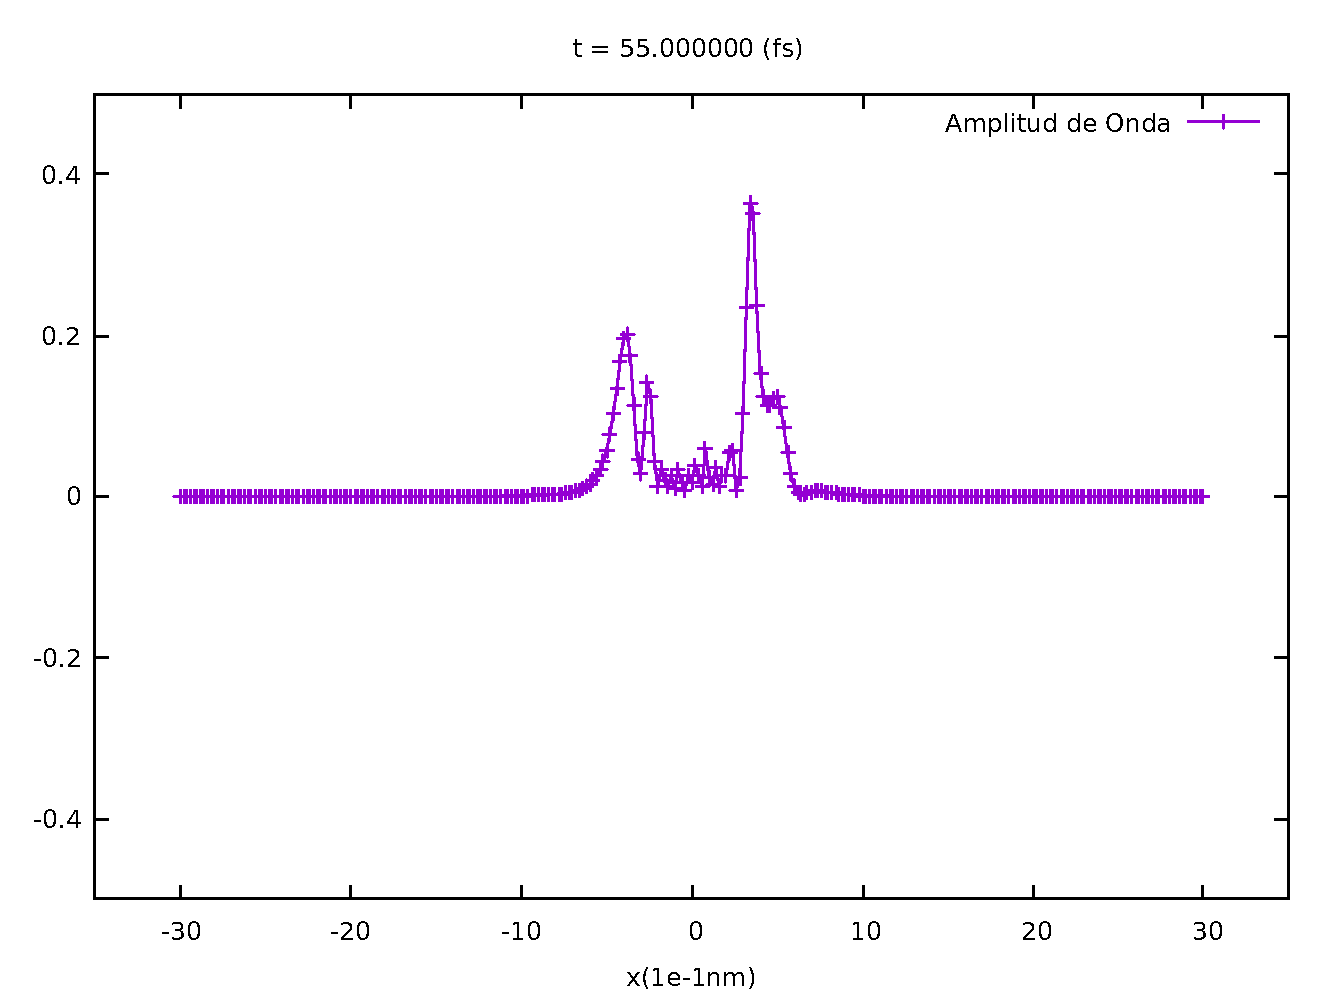
\includegraphics[scale=0.25]{../img/ej7-25_1.pdf}
	\caption{Onda con $E_o = 100eV$.}
	\label{ej7-25_1}
\end{figure}

\begin{figure}[H]
	\centering
	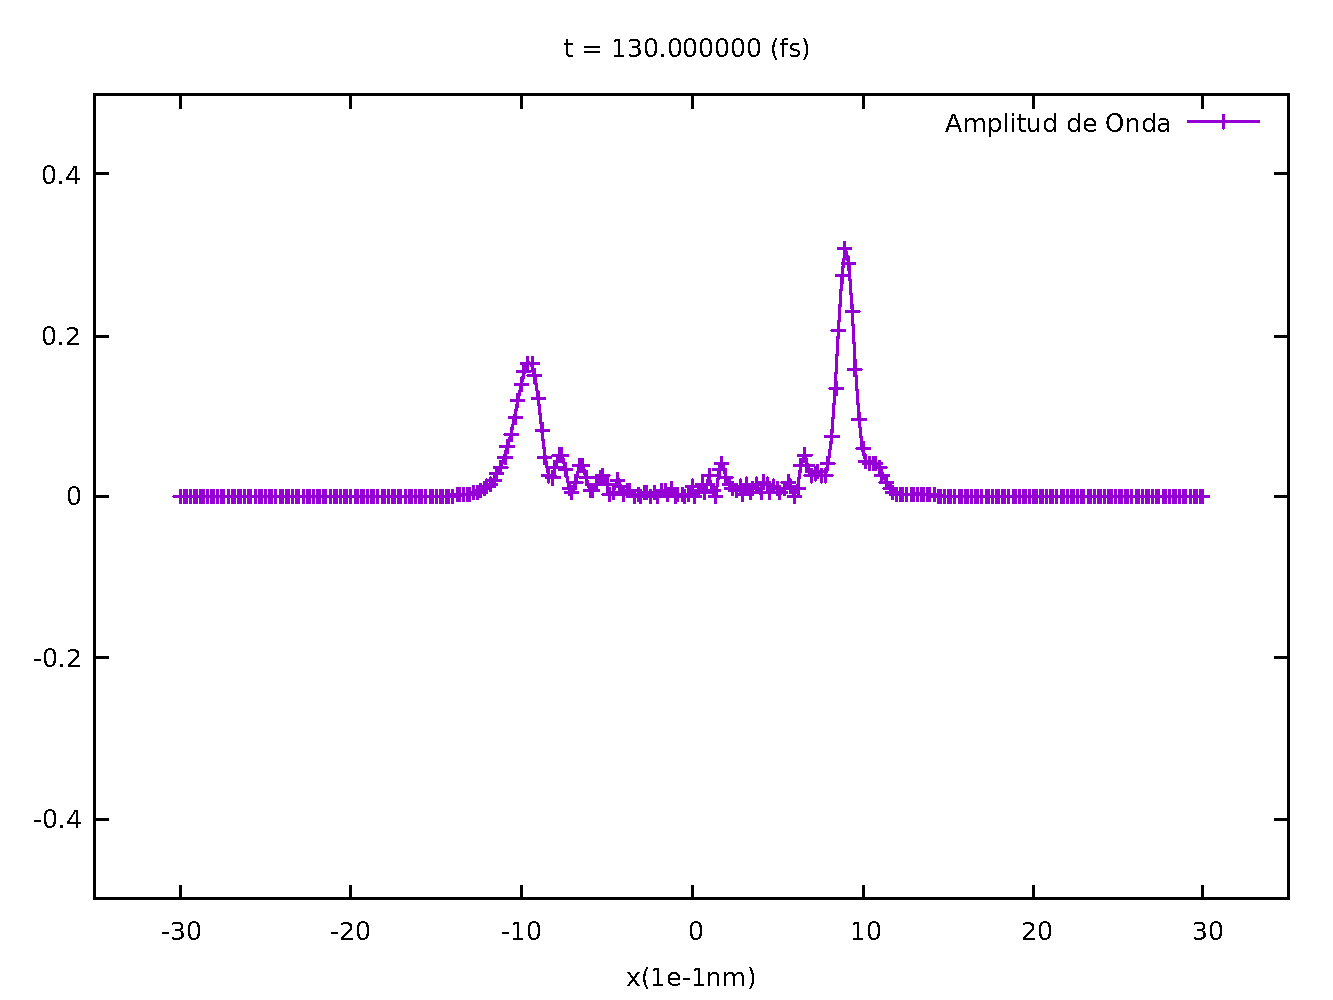
\includegraphics[scale=0.25]{../img/ej7-25_2.pdf}
	\caption{Onda luego de pasar el pozo.}
	\label{ej7-25_2}
\end{figure}
\end{multicols}


\begin{lstlisting}
// Librerias
#include <cmath>
#include <iostream>
#include <fstream>
#include <complex>
#include <iomanip>


using namespace std;



void output( complex<double> *u, double *x, double tiempo, int N, ostream &of );
void fourier( complex<double> *ftrans, complex<double> *f, int n );
void fourierInversa( complex<double> *f, complex<double> *ftrans, int n );


ofstream solucion;
complex<double> I(0.0, 1.0);

int main()
{
  int N = 300;
  int Niter = 30;
  int outCada = 1;
  double tiempo = 0.0;
  double L = 30.0;
  double k0 = 2*M_PI/(N+1);
  double hbar = sqrt(7.6199682);
  double masa = 8.0;
  double dx    = 2*L/N;
  double dt    = 2;
  double delta_x = 1.0; // Ancho del paquete
  double k0momentum = sqrt(2*masa*100)/hbar;  // T=p^2/(2m), p=hbar*k
  double a_potencial = 1.963; //
  solucion.open( "solucion.dat", ios::out );

  // Cantidades complejas
  complex<double> *psi, *trans, *phi, *expV, *expT;
  psi    = new complex<double>[ N+1 ];
  phi    = new complex<double>[ N+1 ];
  trans  = new complex<double>[ N+1 ];
  expV   = new complex<double>[ N+1 ];
  expT   = new complex<double>[ N+1 ];

  // Cantidades reales
  double *x, *k, *V;
  k = new double[ N+1 ];
  x = new double[ N+1 ];
  V = new double[ N+1 ];



  // Inicializar coordenada x
  for(int i=0; i<N+1; i++)
    x[i] = -L + i*dx;

  // Inicializar k
  for(int i=0; i<(N+1)/2; i++)
    k[i] = i*k0;

  for(int i=(N+1)/2; i<N+1; i++)
    k[i] = -k[N+1-i];


  // Inicializar Potencial
  for(int i=0; i<N+1; i++){
    if ( 0<=x[i] && x[i]<=a_potencial )
      V[i] = -200.0;
    else
      V[i] = 0.0;

  }

  // Inicializar expomenciales de T y V
  for(int i=0; i<N+1; i++){
    expV[i] = exp( -I*V[i]*dt/(2*hbar) );
    expT[i] = exp( -I*hbar*k[i]*k[i]*dt/(2*masa) );
  }



  /* condiciones de frontera */
  //psi[0] = 0;
  //psi[N] = 0;


  // condiciones iniciales
  for(int i=0; i<N+1; i++)
    psi[i] = exp(I*k0momentum*x[i] - x[i]*x[i]/pow(2*delta_x,2) )/pow(2*M_PI*pow(delta_x,2),0.25);


  // ciclo principal
  for(int j=0; j<=Niter; j++){

    if ( j%outCada==0 ){
      cout << "it = " << j << " / " << Niter << endl;;
      output( psi, x, tiempo, N, solucion );
    }


    // Aplicacion de los operadores
    for(int i=0; i<N+1; i++)
      phi[i] = expV[i] * psi[i];

    fourier( trans, phi, N+1 );

    for(int i=0; i<N+1; i++)
      phi[i] = expT[i] * trans[i];

    fourierInversa( psi, phi, N+1 );

    for(int i=0; i<N+1; i++)
      psi[i] = expV[i] * psi[i];



    tiempo += dt;

  }

  return 0;
}



/***********************************************************************/




void output( complex<double> *psi, double *x, double tiempo, int N, ostream &of )
{
  for(int i=0; i<N+1; i++)
    of << tiempo << "\t" << x[i] << "\t"  << real(psi[i]) << "\t" << imag(psi[i]) << endl;

  of << endl << endl;
}



void fourier( complex<double> *ftrans, complex<double> *f, int n )
{
  for( int i=0; i<n+1; i++ ){
    ftrans[i] = 0.0;
    for( int j=0; j<n+1; j++ )
      ftrans[i] += f[j] * exp(-2*M_PI*I * (double)j * (double)i / (double)n);

    ftrans[i] /= sqrt(n);
  }
}


void fourierInversa( complex<double> *f, complex<double> *ftrans, int n )
{
  for( int i=0; i<n+1; i++ ){
    f[i] = 0.0;
    for( int j=0; j<n+1; j++ )
      f[i] += ftrans[j] * exp(2*M_PI*I*(double)j*(double)i/(double)n);

    f[i] /= sqrt(n);
  }
}

\end{lstlisting}



















%%%%%%%